\begin{anexosenv}

	\partanexos
	\chapter{Documento de Arquiteruta}
	\label{adoarquitetura}
	\section{introdução}
	Esta documento descreve a arquitetura e tecnologias da aplicação, utilizadas no desenvolvido do sistema de auxilio na detecção da doença de Parkinson utilizando Tremor em repouso. Desenvolvido pelos alunos de Trabalho de Conclusão de Curso 2 da Universidade de Brasília.

	Será desenvolvida uma aplicação web, podendo facilmente ser migrada para uma aplicação mobile em projetos futuros.

	\section{Tecnologias}
	\subsection{Single Page Aplication - SPA}

	\subsection{REST}
	Baseado no baseado no protocolo de comunicação de rede HTTP, sendo simples, rápida e com uma fácil comunicação entre clientes e servidores. Funciona com objetos em formato JSON, e os métodos definidos no protocolo HTTP ( POST, GET, PUT e DELETE) possibilitando assim uma eficiente e rápida troca de informação.

	\section{Representação da Arquitetura}
	A arquitetura se baseia me dois modelos arquiteturais, REST e SPA, interligados com um modelo de aprendizado de máquinas, no caso o Randon Forest ou o SVM, como observado na figura A Figura \ref{diagramadepacotes} na página \pageref{diagramadepacotes}. Ou sejá possui três pacotes:

	\begin{itemize}
		\item Machine Learning models;
		\item API;
		\item Web.
	\end{itemize}


	\subsection{Machine Learning models}
	Consiste no modelo já treinado e vallidado do algoritimo Randon Forest, sendo que este é armazenado no banco de dados \textit{PickleDB}. Deste modo, a comunicação é somente de leitura, com o modelo sendo enviado por completo para a API.
	\subsection{API}
	A API execulta todas as manipulações envolvendo os dados, como o pré-processamento do arquivo enviado pelo usuário, e classificando estes com o modelo salvo. Além de salvar os dados no banco de dados e envia-los quando requisitados, foi desenvolvida utilizadando os padrões de projeto definidos pelo Django-Rest-Framework, possuindo o mair esforço na \textit{View}.

	No caso as seguintes classes foram desenvolvidas, sendo elas:
	\begin{enumerate}
		\item InsertFeature: realiza o cadastro de um paciente.
		\item ListAllPatients: lista todos os pacientes, retornando-os em um objeto JSON.
		\item DetailPatient: retorna os detalhes relativos a um único paciente.
		\item UpdatePatient: possibilita a edição de um paciente já cadastrado.
		\item CLS: possui apenas um método GET, que recebe um id de um paciente. Com auxilio de outros métodos carrega o arquivo sEMG associado a este paciente, realiza o pré-processamento aplicando a FFT, carrega o modelo e por fim retorna o resultado da classificação.
	\end{enumerate}

	\subsection{Web}
	Responsável pela exibição dos dados, desenvolvido em react. Possui somente três componentes, cadastrado, editar e home.

	\section{Restrições e Metas Arquiteturais}
	\section{Visão Lógica}
	\subsection{Diagrama de Classes}
	\subsection{Diagrama de Pacotes}
	\begin{figure}[!htb]
		\centering
		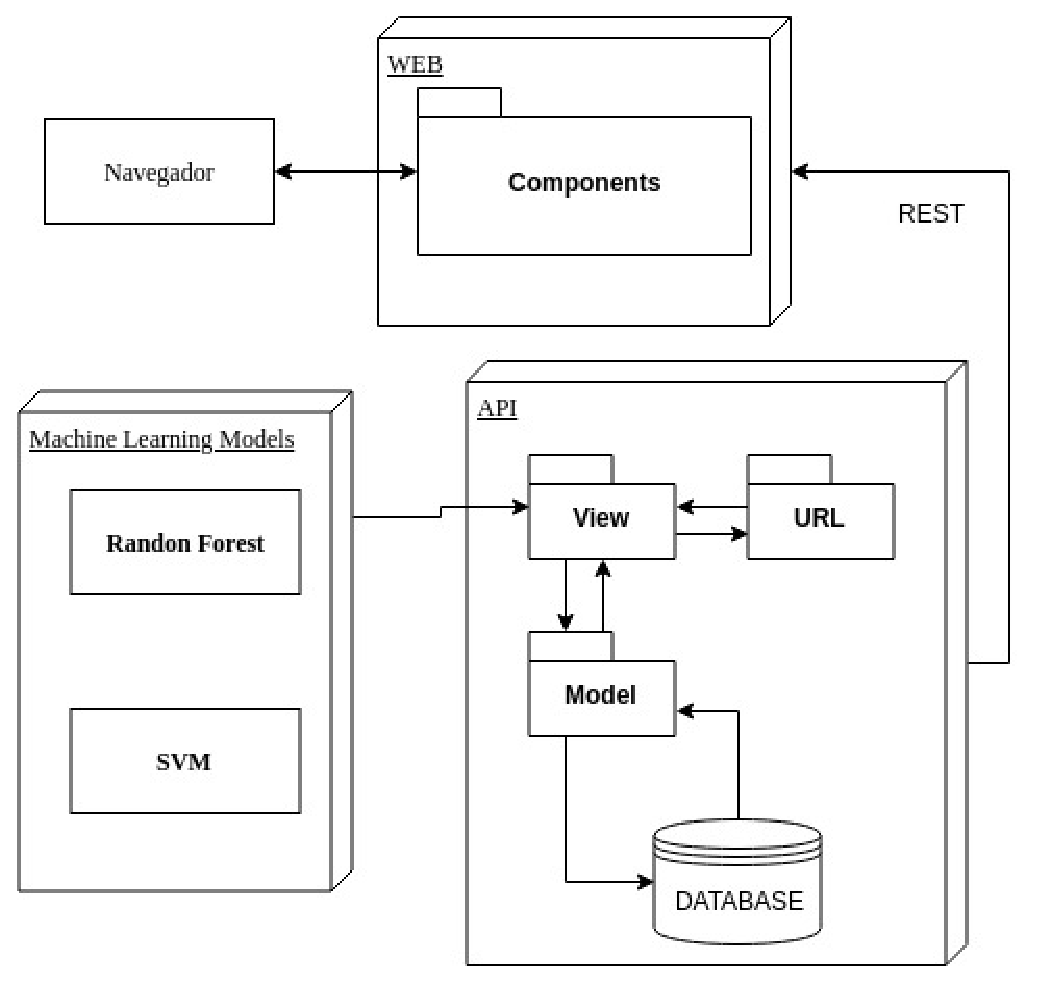
\includegraphics[width=0.9\textwidth]{figuras/diagrama_pacotes.eps}
		\caption{Diagrama de pacotes}
		\label{diagramadepacotes}
	\end{figure}

	\section{Referências}
	% \partanexos

	% \includepdf[pages=-,pagecommand=\chapter{Protocolo PKS}]{./Protocolo_PKS.pdf}

	\chapter[Documento de Visão]{Documento de Visão}
	\label{adocvisao}

	\section{Introdução}

	Este documento tem como propósito descrever todos os requisitos de um sistema capaz de realizar um diagnóstico preliminar da doença de Parkinson em pacientes com suspeita de serem portadores da mesma, denominado Detector preliminar da Doença de Parkinson(DPDP). Serão explicitados os aspectos inerentes ao sistema, visando uma melhor definição do projeto de forma simplificada. O documento está organizado em 8 tópicos que visam uma melhor compreensão do leitor, sendo eles: introdução, posicionamento, descrição da parte interessada e do usuário, visão geral do produto, recursos do produto, restrições. Em todos os tópicos são abordados pontos cruciais para o desenvolvimento do projeto.

	\subsection{Problema}

	Atualmente o diagnóstico da doença de Parkinson é feito avaliando-se a história do paciente, o seu exame neurológico, resposta à terapia dopaminérgica e avaliação dos sinais obtidos por dispositivos sEMG, esses métodos, apesar de eficazes, ainda demandam um certo tempo para alcançar o diagnóstico concreto da doença. Portanto o desenvolvimento de um sistema utilizando aprendizagem de máquina torna-se um viés mais eficaz para auxiliar nessas etapas do diagnóstico da doença de Parkinson.

	\subsection{Escopo}

	O DPDP permite que o médico (usuário) possa fazer uma avaliação preliminar prévia do estado do paciente quanto a presença ou não da doença de Parkinson inserindo dados obtidos por um dispositivo sEMG. O sistema também permite que o médico consulte no banco de dados os pacientes que já seu diagnóstico preliminar.

	\section{Posicionando}

	\subsection{Oportunidade de Negócios}

	Apesar dos meios para o diagnóstico da doença de Parkinson serem considerados suficientes, o desenvolvimento de um sistema capaz de melhorar ainda mais essa eficiência desse diagnóstico utilizando os conceitos do aprendizado de máquina, ainda tendo em vista que não existem outros meios semelhantes a esse sistema para aferir um diagnóstico preliminar da doença, pode significar um passo a mais no quesito diagnóstico não apenas da doença de parkinson, mas também de outros distúrbios neurológicos.

	\subsection{Instrução do Problema}

	\begin{table}[]
		\centering
		\caption{Instrução do Problema}
		\begin{tabular}{|c|c|}
			\hline
			\textbf{O problema}            & Baixa eficiência do diagnóstico da doença de Parkinson                           \\ \hline
			\textbf{Afeta}                 & Os pacientes                                                                     \\ \hline
			\textbf{Cujo o impacto é}      & Um possível diagnóstico tardio da doença                                         \\ \hline
			\textbf{Uma boa solução seria} & Sistema automatizado capaz fornecer um diagnóstico prévio da doença de Parkinson \\ \hline
		\end{tabular}
		\label{table:Instrução do Problema}
	\end{table}

	\section{Descrições da Parte Interessada e do Usuário}

	\subsection{Resumo da Parte Interessada}

	\begin{table}[]
		\centering
		\caption{Resumo da Parte Interessada}
		\begin{tabular}{@{}|l|l|l|@{}}
			\toprule
			\textbf{Nome\textbackslash{}} & \textbf{Descrição}                             & \textbf{Responsabilidade}                                                                                                        \\ \midrule
			\textbf{Orientandos}          & Estudantes matriculados na disciplina de TCC 2 & Desenvolvimento da solução de software e pesquisa                                                                                \\ \midrule
			\textbf{Orientadores}         & ...                                            & Orientadores e avaliadores que darão suporte a respeito das pesquisas e escrita do TCC assim como no desenvolvimento do sistema. \\ \bottomrule
		\end{tabular}
		\label{table:Resumo da Parte Interessada}
	\end{table}

	\subsection{Resumo do Usuário}

	\begin{table}[]
		\centering
		\caption{Resumo do Usuário}
		\begin{tabular}{@{}|l|l|l|@{}}
			\toprule
			\textbf{Nome\textbackslash{}} & \textbf{Descrição}                   & \textbf{Responsabilidade}                                                                           \\ \midrule
			\textbf{Médicos}              & Pessoas capacitadas da área da saúde & Inserir os dados dos pacientes, verificar o diagnóstico e consultar os dados dos pacientes no banco \\ \bottomrule
		\end{tabular}
		\label{table:Resumo do Usuário}
	\end{table}

	\subsection{Perfis das Partes Interessadas}

	\subsubsection{Orientandos}

	\begin{table}[]
		\centering
		\caption{Perfil dos Orientandos}
		\begin{tabular}{@{}|l|l|@{}}
			\toprule
			\textbf{Representantes}       & Flávio da Costa Paixão, Jônnatas Lennon Lima Costa                                                \\ \midrule
			\textbf{Descrição}            & Desenvolvedores do sistema e gerenciamento do projeto                                             \\ \midrule
			\textbf{Tipo}                 & Estudantes matriculados na disciplina de TCC 2                                                    \\ \midrule
			\textbf{Responsabilidades}    & Desenvolvimento da solução de software e pesquisa                                                 \\ \midrule
			\textbf{Critérios de Sucesso} & Manter os prazos estabelecidos sem atraso, e gerenciar a qualidade do software em desenvolvimento \\ \midrule
			\textbf{Envolvimento}         & Alto                                                                                              \\ \bottomrule
		\end{tabular}
		\label{table:Perfil dos Orientandos}
	\end{table}

	\subsubsection{Orientadores}

	\begin{table}[]
		\centering
		\caption{Perfil dos Orientadores}
		\begin{tabular}{@{}|c|c|@{}}
			\toprule
			\textbf{Representantes}       & Dra. Lourdes Mattos Brasil, MSc. Roberto Aguiar Lima                                                                             \\ \midrule
			\textbf{Descrição}            & ...                                                                                                                              \\ \midrule
			\textbf{Tipo}                 & Orientadores e avaliadores que darão suporte a respeito das pesquisas e escrita do TCC assim como no desenvolvimento do sistema. \\ \midrule
			\textbf{Responsabilidades}    & Orientar e avaliar                                                                                                               \\ \midrule
			\textbf{Critérios de Sucesso} & Olhar crítico na avaliação do projeto                                                                                            \\ \midrule
			\textbf{Envolvimento}         & Alto                                                                                                                             \\ \bottomrule
		\end{tabular}
		\label{table:Perfil dos Orientadores}
	\end{table}

	\subsection{Perfis do Usuário}

	\subsubsection{Médicos}

	\begin{table}[h] \footnotesize
		\centering
		\caption{Perfil dos Médicos}
		\begin{tabular}{@{}|c|c|@{}}
			\toprule
			\textbf{Representantes}       & Médicos                                                                                                                                                                                \\ \midrule
			\textbf{Descrição}            & Pessoa capacitada para verificar o diagnóstico da doença de Parkinson em seus pacientes                                                                                                \\ \midrule
			\textbf{Tipo}                 & Profissionais que tem o interesse em utilizar o sistema para validar um diagnóstico preliminar da doença de parkinson em seus pacientes.                                               \\ \midrule
			\textbf{Responsabilidades}    & Verificar o diagnóstico do paciente através do sistema                                                                                                                                 \\ \midrule
			\textbf{Critérios de Sucesso} & Manter-se ciente de que o diagnóstico é preliminar e serve apenas como ferramenta de auxílio para a identificação de alguns padrões que podem indicar a presença da doença no paciente \\ \midrule
			\textbf{Envolvimento}         & Alto                                                                                                                                                                                   \\ \bottomrule
		\end{tabular}
		\label{table:Perfil dos Médicos}
	\end{table}

	\section{Descrição da Solução}

	\subsection{Perspectiva do Produto}

	O sistema tem como objetivo utilizar os sinais obtidos por um dispositivo sEMG para realizar um diagnóstico preliminar da doença de Parkinson utilizando um modelo de aprendizado de máquina.

	\subsection{Resumo dos recursos}

	\begin{table}[]
		\centering
		\caption{Resumo dos recursos}
		\begin{tabular}{@{}|c|c|@{}}
			\toprule
			\textbf{Benefício para o cliente}                & \textbf{Recursos de suporte}                                                                                    \\ \midrule
			Automatizar o processo de diagnóstico preliminar & O sistema permite a inclusão dos dados gerados pelos dispositivos sEMG para a verificação da presença da doença \\ \midrule
			Manter registro de pacientes no banco de dados   & O sistema possibilita a consulta de pacientes já diagnosticados preliminarmente                                 \\ \bottomrule
		\end{tabular}
		\label{table:Resumo dos recursos}
	\end{table}

	\subsection{Recursos do Produto}

	O sistema DPDP oferece as seguintes funcionalidades:

	\begin{itemize}
		\item Incluir os dados do paciente
		\item Realizar diagnóstico preliminar da doença de Parkinson
		\item Consultar dados dos pacientes já diagnosticados preliminarmente
		\item Arquivar dados dos pacientes
		\item Editar dados dos pacientes
	\end{itemize}

	\subsection{Requisitos Funcionais}

	\begin{table}[]
		\centering
		\caption{Requisitos Funcionais}
		\begin{tabular}{@{}|c|c|@{}}
			\toprule
			\textbf{ID} & \textbf{Descrição}         \\ \midrule
			RF01        & Cadastrar paciente         \\ \midrule
			RF02        & Editar paciente            \\ \midrule
			RF03        & Consultar paciente         \\ \midrule
			RF04        & Arquivar paciente          \\ \midrule
			RF05        & Baixar dados do paciente   \\ \midrule
			RF06        & Imprimir lista de paciente \\ \midrule
			RF07        & Fazer upload de arquivos   \\ \midrule
			RF08        & Diagnóstico preliminar     \\ \bottomrule
		\end{tabular}
		\label{table:Requisitos Funcionais}
	\end{table}


\end{anexosenv}
